\documentclass[12pt,answers]{exam}

\usepackage{amsmath,amsfonts,amssymb,mathtools,physics,commath}
\usepackage{todonotes}
\usepackage{float}
\usepackage{multicol}
\usepackage{polynom}
\usepackage{siunitx}

\newcommand{\inv}{^{-1}}

\pagestyle{headandfoot}
\firstpageheadrule
\runningheadrule
\firstpageheader{Math 221}{Final Exam|Solutions, Page \thepage\ of \numpages}{May 15, 2019}
\runningheader{Math 221}{Final Exam|Solutions, Page \thepage\ of \numpages}{May 15, 2019}
\runningfooter{}{}{}

\begin{document}
% \maketitle
\begin{questions}
\question Evaluate the following integrals.
\begin{parts}
    \part[10]
    $\displaystyle \int x^3 \ln(x) \dif x$
    \begin{solution}
        \[
            \begin{array}{ccc}
                & D & I \\ 
                + & \ln x & x^3 \\ 
                - & \dfrac 1x & \dfrac{x^4}{4}
            \end{array}
        \]
        so
        \begin{align*}
            \int x^3 \ln(x) \dif x
            = \frac{x^4}{4} \ln x - \int \frac14 x^3 \dif x
            = \boxed{\frac{x^4}{4} \ln x - \frac{1}{16} x^4 + C}
        \end{align*}
    \end{solution}
    \part[12]
    $\displaystyle \int \frac{x^2 \dif x}{\sqrt{x^2-1}}$
    \begin{solution}
        $x = \sec \theta$, $\dif x = \sec \theta \tan\theta \dif \theta$.
        \begin{multicols}{2}
        \begin{align*}
            \int \frac{x^2}{\sqrt{x^2-1}} \dif x
            &= \int \frac{\sec^2 \theta}{\sqrt{\sec^2 \theta - 1}} \sec \theta \tan \theta \dif \theta \\ 
            &= \int \frac{\sec^2 \theta}{\sqrt{\tan^2 \theta}} \sec \theta \tan \theta \dif \theta \\ 
            &= \int \frac{\sec^2 \theta}{\tan \theta} \sec \theta \tan \theta \dif \theta \\ 
            &= \int \sec^3 \theta \dif \theta \\ 
            &= \frac{\sec \theta \tan \theta}{2} + \frac12 \int \sec \theta \dif \theta \\ 
            &= \frac{\sec \theta \tan \theta}{2} + \frac12 \ln|\sec \theta + \tan \theta|  \\
            &= \frac{\sec \theta \tan \theta}{2} + \frac12 \ln|\sec \theta + \tan \theta| \\
            &= \boxed{\frac12 x \sqrt{x^2-1} + \frac12 \ln \abs{x + \sqrt{x^2-1}} + C}
        \end{align*}
        \begin{figure}[H]
            \centering
            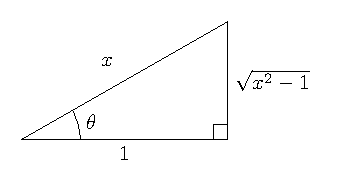
\includegraphics{graphics/2019-spring-final-1b.pdf}
        \end{figure}
        \end{multicols}
    \end{solution}
\end{parts}

\newpage
\question Evaluate the integrals.
\begin{parts}
    \part[10]
    $\displaystyle \int \frac{e^x}{\sqrt{4-e^{2x}}} \dif x$
    \begin{solution}
        $u = e^x$, $\dif u = e^x \dif x$,
        \begin{align*}
            \int \frac{e^x}{\sqrt{4-e^{2x}}} \dif x 
            &= \int \frac{1}{\sqrt{4-u^2}} \dif u  \\
            &= \sin[-1](\frac u2) \\ 
            &= \boxed{\sin[-1](\frac{e^x}{2}) + C}
        \end{align*}
    \end{solution}
    \part[12]
    $\displaystyle \int \frac{x^2-4}{x^3+x} \dif x$
    \begin{solution}
        \[
            \frac{x^2-4}{x(x^2+1)} = \frac{-4}{x} + \frac{5x}{x^2+1}
        \]
        so
        \begin{align*}
            \int \frac{x^2-4}{x^3+x} \dif x 
            &= \int \left( \frac{-4}{x} + \frac{5x}{x^2+1} \right) \dif x \\ 
            &= \boxed{-4 \ln|x| + \frac 52 \ln(x^2+1) + C}
        \end{align*}
    \end{solution}
\end{parts}

\question[10]
Evaluate the improper integral or show that it diverges
$\displaystyle \int_0^\infty x e^{-2x^2} \dif x$
\begin{solution}
$u = -2x^2$, $\dif u = -4 x \dif x$. 
so
\begin{align*}
    \int_0^\infty x e^{-2x^2} \dif x
    &= -\frac 14 \int_0^{-\infty} e^{u} \dif u \\ 
    &= \frac14 \eval{e^{u}}_{-\infty}^0 \\
    &= \frac14 \left[ e^0 - \lim_{b\to-\infty} e^b \right] \\ 
    &= \frac14 \left( 1 - 0 \right) 
    = \boxed{\frac14}
\end{align*}
\end{solution}

\newpage
\question
Let $R$ be the region trapped between $y = 1$ and $y = \cos x$ with $0 \le x \le \dfrac\pi2$.
\begin{parts}
    \part[6] Find the area of the region $R$.
    \begin{solution}
        \begin{align*}
            \int_0^{\pi/2} (1 - \cos x) \dif x
            &= \eval{x - \sin x}_0^{\pi/2} \\
            &= \frac\pi2 - 1 - (0)
            = \boxed{\frac\pi2 - 1}
        \end{align*}
    \end{solution}
    \part[10] Find $\overline x$, the $x$ coordinate of the centroid of $R$. (Do not calculate $\overline y$.)
    \begin{solution}
        \begin{multicols}{2}
        \begin{align*}
            M_y &= \int_0^{\pi/2} x (1 - \cos x) \dif x \\
            &= \eval{\frac{x^2}{2} - (x \sin x + \cos x) }_0^{\pi/2} \\ 
            &= \left(\frac{\pi^2}{8} - \frac\pi2 \right) -(-1) \\
            &= \boxed{\frac{\pi^2}{8} - \frac\pi2 + 1}
        \end{align*}
        \[
            \begin{array}{ccc}
                & D & I \\ 
                + & x & \cos x \\ 
                - & 1 & \sin x \\ 
                + & 0 & -\cos x
            \end{array}
        \]
        \end{multicols}
    \end{solution}
\end{parts}

\question[8] Evaluate the series $\displaystyle \sum_{n=1}^\infty \sin(\frac\pi2 n) 2^{-n}$
\begin{solution}
    Notice that $\sin(\frac\pi2 n)$ cycles between the values $1, 0, -1, 0$. Expanding out the series:
    \begin{align*}
\sum_{n=1}^\infty \sin(\frac\pi2 n) 2^{-n}
        &= 1 \cdot 2^{-1} + 0 \cdot 2^{-2} + (-1) \cdot 2^{-3} + 0 \cdot 2^{-4} \\ 
        &\quad + 1 \cdot 2^{-5} + 0 \cdot 2^{-6} + (-1) \cdot 2^{-7} + 0 \cdot 2^{-8} + \cdots \\
        &= 2^{-1} - 2^{-3} + 2^{-5} - 2^{-7} + \cdots \\
        \intertext{which is a geometric series with $a = 2^{-1}$ and $r = -2^{-2}$, converging to}
        &= \frac{\frac12}{1 - (-\frac14)}
        = \frac 12 \cdot \frac 45 
        = \boxed{\frac 25}
    \end{align*}
\end{solution}

\question Let $\displaystyle S = \sum_{n=1}^\infty \frac{(-1)^n}{n!}$.
\begin{parts}
    \part[4] Explain why the series converges.
    \begin{solution}
        \todo[inline]{write better?}
        Can use Direct Comparison Test to argue, since
        \[
            \frac{1}{n!} \le \frac{1}{n^2} \text{ for } n \ge 4
            \quad \text{ and } \quad
            \sum \frac{1}{n^2} \text{ converges}
        \]
        or can use Ratio Test, since
        \[
            \lim_{n\to\infty} \frac{\frac{1}{(n+1)!}}{\frac{1}{n!}}
            = \lim_{n\to\infty} \frac{n!}{(n+1)!}
            = \lim_{n\to\infty} \frac{1}{n+1} = 0
        \]
    \end{solution}
    \part[4] How many terms are required to approximate $S$ with an error less than 0.01?
    \begin{solution}
        Error for alternating series:
        \[
            |S - S_N| = \frac{1}{(N+1)!} < 0.01
            \implies 100 < (N+1)! 
        \]
        This holds once $\boxed{N \ge 5}$
    \end{solution}
    \part[2] Evaluate $S$ by using an appropriate series on the cover page.
    \begin{solution}
        \begin{align*}
            e^x &= \sum_{n=0}^\infty \frac{x^n}{n!} \\ 
            e^{-1} &= \sum_{n=0}^\infty \frac{(-1)^n}{n!} \\ 
            &= 1 + \sum_{n=1}^\infty \frac{(-1)^n}{n!} \\ 
            \implies \boxed{e^{-1} - 1} &= \sum_{n=1}^\infty \frac{(-1)^n}{n!}  
        \end{align*}
    \end{solution}
\end{parts}

\newpage
\question[12]
Solve the initial value problem, $\displaystyle \dod{y}{t} = \frac{\cos^2(y)}{e^{2t}}$, $y(0) = 0$. Express your final answer in the form $y = f(t)$.
\begin{solution}
    \begin{align*}
        \int \sec^2(y) \dif y &= \int e^{-2t} \dif t \\ 
        \tan(y) &= -\frac12 e^{-2t} + C \\ 
        y(t) &= \boxed{\tan[-1](-\frac12 e^{-2t} + C)}
    \end{align*}
\end{solution}

\question[12]
Find the interval of converge of the power series $\displaystyle \sum_{n=1}^\infty \frac{(x+2)^n}{\sqrt n \cdot 3^n}$.
(Make clear the status of any end points.)
\begin{solution}
    \todo[inline]{check over this later}
    \begin{align*}
        \rho &= \lim_{n\to\infty} \left| \frac{(x+2)^{n+1}}{\sqrt{n+1} \cdot 3^{n+1}} \cdot \frac{\sqrt n \cdot 3^n}{(x+2)^n} \right| \\ 
        &= \lim_{n\to\infty} \left| \frac{x+2}{3} \frac{\sqrt{n}}{\sqrt{n+1}} \right| \\
        &= \frac13 |x+2| < 1
    \end{align*}
    Radius of convergence : 3, centered at $x = -2$. 
    \\
    For $x = 1$: 
    \[
        \sum_{n=1}^\infty \frac{3^n}{\sqrt n \cdot 3^n}
        = 
        \sum_{n=1}^\infty \frac{1}{\sqrt n } \text{ diverges by $p$-series test}
    \]
    For $x = -5$:
    \[
        \sum_{n=1}^\infty \frac{(-3)^n}{\sqrt n \cdot 3^n}
        = 
        \sum_{n=1}^\infty \frac{(-1)^n}{\sqrt n} \text{ converges by AST}
    \]
    Thus the interval of convergence is $\boxed{\intco{-5, 1}}$.
\end{solution}

\newpage
\question
Determine whether the following series converge or diverge.
State clearly which test you are using and implement the test as clearly as you can.
The answer for each problem is worth 2 points and the work you show 4 points.
\begin{parts}
    \part[6]
    $\displaystyle \sum_{n=3}^\infty \frac{1+\frac1n}{7 \cos \frac 1n}$
    \begin{solution}
        \fbox{Diverges} by divergence test, since $\displaystyle \lim_{n\to\infty} \frac{1+\frac1n}{7 \cos \frac 1n} = \frac 17 \ne 0$
    \end{solution}
    \part[6]
    $\displaystyle \sum_{n=2}^\infty \frac{n^2 + 5}{n^{5/2} + n}$
    \begin{solution}
        Limit comparison test with $\displaystyle \sum \frac{1}{n^{1/2}}$. Then 
        \[
            \lim_{n\to\infty} 
            \frac{\dfrac{n^2 + 5}{n^{5/2} + n}}{\dfrac{1}{n^{1/2}}}
            = 
            \lim_{n\to\infty} 
            \frac{n^{5/2} + 5n^{1/2}}{n^{5/2} + n} = 1 
            \quad \text{and} \quad \sum \frac{1}{n^{1/2}} \text{ diverges by $p$-series test}
        \]
        So by Limit Comparison Test, 
$\displaystyle \sum_{n=2}^\infty \frac{n^2 + 5}{n^{5/2} + n}$ \fbox{diverges}
    \end{solution}
    \part[6]
    $\displaystyle \sum_{n=1}^\infty \frac{(n!)^2}{(2n)!}$
    \begin{solution}
        Using the Ratio Test:
        \[
            \lim_{n\to\infty} \left| \frac{((n+1)!)^2}{(2(n+1))!} \cdot \frac{(2n)!}{(n!)^2} \right|
        = 
            \lim_{n\to\infty} \left| \frac{(n+1)^2}{(2n+2)(2n+1)} \right|
            = \frac 14
        \]
        Thus by the Ratio Test, the series \fbox{converges}
    \end{solution}
\end{parts}

\newpage
\question[12]
Find the second degree Taylor polynomial $T_2(x)$ for the function $f(x) = \sqrt{x}$ centered at $x = 4$.
\begin{solution}
    Recall the formula for the $n$th Taylor polynomial centered at $x=a$:
        \begin{align*}
            T_n(x) &= f(a) + f'(a) (x-a) + \frac{f''(a)}{2!} (x-a)^2 + \cdots + \frac{f^{(n)}(a)}{n!} (x-a)^n 
        \end{align*}
        Thus we compute
        \begin{align*}
            f(x) &= \sqrt x
           & f(4) &= 2 \\ 
           f'(x) &= \frac{1}{2\sqrt x} = \frac12 x^{-1/2}
           & f'(4) &= \frac{1}{4} \\ 
           f''(x) &= -\frac{1}{4}x^{-3/2} = -\frac{1}{4 x^{3/2}}
           & f''(4) &= -\frac{1}{4 \cdot 8}
        \end{align*}
        so
        \[
            T_2(x) = \boxed{2 + \frac14 (x-4) - \frac{1}{64}(x-4)^2}
        \]
\end{solution}

\newpage
\question
\begin{parts}
    \part[4] Use an approximate series from the cover sheet to find the Maclaurin series for $\dfrac{1}{1+x^2}$
    \begin{solution}
        Starting with
        \begin{align*}
            \frac{1}{1-x} &= \sum_{n=0}^\infty x^n \\
            \shortintertext{we substitute to get}
            \frac{1}{1-(-x^2)} 
            = \frac{1}{1+x^2} 
            &= \sum_{n=0}^\infty (-x^2)^{n} 
            = \boxed{\sum_{n=0}^\infty (-1)^n x^{2n}}
        \end{align*}
    \end{solution}
    \part[4] By integrating your expansion in part (a) obtain the Maclaurin series for $\tan\inv x$.
    \begin{solution}
        Dropping integrals:
        \begin{align*}
            \int \frac{1}{1+x^2} \dif x 
            &= \int \sum_{n=0}^\infty (-1)^n x^{2n} \dif x \\
            \implies \tan\inv x 
            &= \sum_{n=0}^\infty \int (-1)^n x^{2n} \dif x
            = \boxed{\sum_{n=0}^\infty \frac{(-1)^n}{2n+1} x^{2n+1} }
        \end{align*}
    \end{solution}
    \part[2] Use part (b) to evaluate the sum $1 - \frac 13 + \frac 15 - \frac 17 + \frac 19 - \cdots = $
    \begin{solution}
        Evaluating the Maclaurin series in (b) at $x=1$ gives the sum specified. Thus
        \[
            1 - \frac 13 + \frac 15 - \frac 17 + \frac 19 - \cdots = \tan\inv(1) = \boxed{\frac\pi4}
        \]
    \end{solution}
\end{parts}

\newpage
\question[8]
Use the series
\begin{alignat*}{2}
    e^x      & = \sum_{n=0}^\infty \frac{x^n}{n!}
             &                                              & = 1 + x + \frac{x^2}{2} + \cdots         \\
    \intertext{and}
    \ln(1+x) & = \sum_{n=1}^\infty (-1)^{n+1} \frac{x^n}{n}
             &                                              & = x - \frac12 x^2 + \frac13 x^3 - \cdots
\end{alignat*}
to find the terms up to $x^4$ for the Maclaurin series of $e^{2x} \ln(1+x^2)$.
\begin{solution}
\begin{align*}
    e^{2x} \ln(1+x^2) 
    &= \left( \sum_{n=0}^\infty \frac{(2x)^n}{n!} \right) \left( \sum_{n=1}^\infty (-1)^{n+1} \frac{x^{2n}}{n}\right) \\ 
    &= \left(1 + 2x + \frac{(2x)^2}{2} + \frac{(2x)^3}{6} + \cdots \right) \left( x^2 - \frac12 x^{4} + \frac13 x^6 + \cdots \right) \\ 
    &= \left(x^2 - \frac12 x^4 + \cdots \right) + \left(2x^3 + \cdots \right) + \left( 2x^4 + \cdots \right) + \cdots \\ 
    &= \boxed{x^2 + 2x^3 + \frac 32 x^4} + \text{h.o.t.}
\end{align*}
\end{solution}

\newpage
\question
\begin{parts}
    \part[6]
    Sketch the graph of the polar equation $r = 6 \cos(\theta)$, $0 \le \theta \le \pi$.
    \begin{solution}
        \begin{figure}[H]
            \centering
            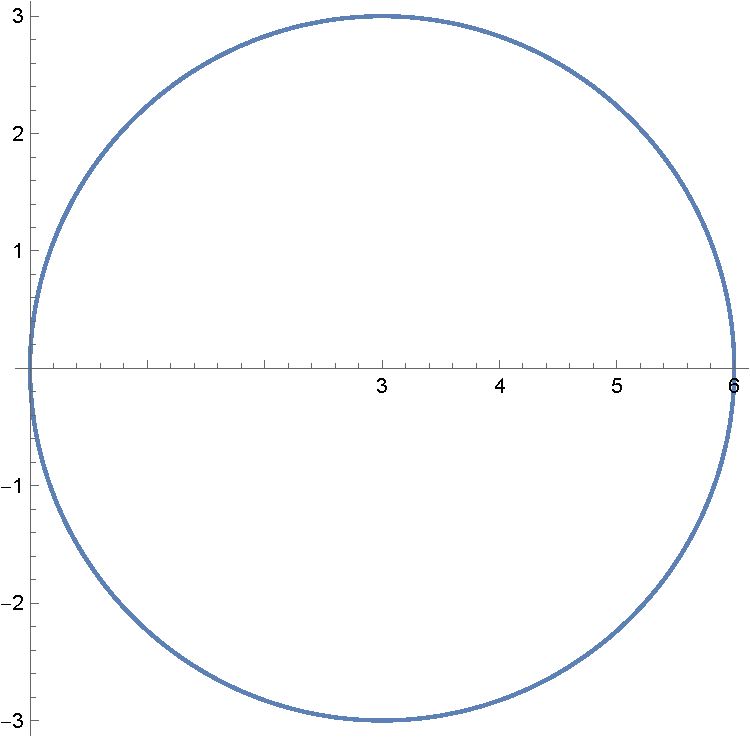
\includegraphics[width=.3\textwidth]{graphics/2019-spring-final-13a.pdf}
        \end{figure}
    \end{solution}
    \part[6]
    Convert the polar equation in part (a) to a rectangular equation in $x$ and $y$, and state what familiar shape it is?
    \begin{solution}
        The formulas used to switch to polar are
        \[
            r = \sqrt{x^2+y^2} \qquad x = r \cos \theta 
        \]
        Converting to rectangular:
        \begin{align*}
            r &= 6 \cos(\theta) \\ 
 \sqrt{x^2+y^2} &= 6  \frac{x}{\sqrt{x^2+y^2}} \\ 
            x^2 + y^2 &= 6x \\
            x^2 - 6x + 9 + y^2 &= 9 \\ 
            (x-3)^2 + y^2 &= 3^2
        \end{align*}
        This is a \fbox{circle of radius 3 centered at $(3, 0)$}
    \end{solution}
\end{parts}

\newpage
\question
Consider the curve with parametric equations $x = 4-\sin(2t)$, $y = 5+\cos(2t)$.
\begin{parts}
    \part[6]
    Find the slope of the curve at a general value of $t$.
    \begin{solution}
        \begin{align*}
        \frac{\dif y}{\dif x} 
        = \frac{\dod{y}{t}}{\dod{x}{t}} 
        = \frac{-2\sin(2t)}{-2\cos(2t)} 
        = \boxed{\tan(2t)}
        \end{align*}
    \end{solution}
    \part[4]
    Find the equation of the tangent line to the curve at $t = \pi/2$.
    \begin{solution}
        Computing:
        \begin{align*}
        m = \dod{y}{x}(\pi/2) = \tan(\pi) = 0 \\
        x(\pi/2) = 4 - \sin(\pi) = 4 \\ 
        y(\pi/2) = 5 + \cos(\pi) = 4
        \end{align*}
        The tangent line is $\boxed{y = 4}$
    \end{solution}
    \part[8]
    Find the length of the curve for $0 \le t \le \pi$.
    \begin{solution}
        \begin{align*}
            L &= \int_0^\pi \sqrt{\left(\dod{x}{t}\right)^2 + \left(\dod{y}{t}\right)^2} \dif t \\ 
            &= \int_0^\pi \sqrt{4\cos^2(2t) + 4\sin^2(2t)} \dif t \\
            &= \int_0^\pi \sqrt 4 \dif t 
            = \boxed{2\pi}
        \end{align*}
    \end{solution}
\end{parts}

\newpage
\question[10]
Calculate the area bounded by one petal of the rose $r = 2\cos(4\theta)$.
\begin{solution}
    We need to determine the interval for $\theta$ that traces out a single petal. 
    A single lobe for $\cos \theta$ occurs in the interval $\theta \in [-\frac\pi2, \frac\pi2]$.
    Relating this to the given function, we require
    \begin{align*}
        4\theta = -\frac\pi2 &\implies \theta = -\frac\pi8 \\ 
        4\theta = \frac\pi2 &\implies \theta = \frac\pi8 
    \end{align*}
    Thus the interval is $\theta \in [-\frac\pi8, \frac\pi8]$

    The area (in polar) is given by
    \begin{align*}
        A = \int_\alpha^\beta \frac12 r^2 \dif \theta
        &= \int_{-\pi/8}^{\pi/8} \frac12 (2\cos(4\theta))^2 \dif \theta\\ 
        &= \int_{-\pi/8}^{\pi/8} 2 \cos^2(4\theta) \dif \theta & (u = 4\theta; \dif u = 4\dif \theta)\\
        &= \frac 12 \int_{-\pi/2}^{\pi/2} \cos^2(u) \dif u \\
        &= \int_{0}^{\pi/2} \cos^2(u) \dif u & (\text{symmetry of even functions})\\
        &= \frac12 \sin u \cos u + \frac 12 \int 1 \dif u \\ 
        &= \frac12 \bigl[\sin u \cos u + u \bigr]_0^{\pi/2} \\
        &= \frac12\left[ \left(0 + \frac\pi2 \right) - 0 \right]
        = \boxed{\frac \pi4}
    \end{align*}
\end{solution}
\end{questions}
\end{document}